\documentclass[../main.tex]{subfiles} % To be correctly processed by subfiles

% Do not use any packages here, write imports directly to main.tex

\begin{document}


\subsection{ICA}

Independent Component Analysis (ICA) is a method developed particularly for solving a blind source separation problem, although it might also be used for dimensionality reduction. 
A very good explanation of ICA is given at [3], here we briefly provide the intuition and pseudocode.

It acts similarly to Principal Component Analysis in a sense that they both try to find a basis set of vectors of the data that optimizes some property. 
The difference is that instead of making the components orthogonal by requiring them to explain the maximum possible variance along each axis, it tries to make them as independent as possible:

\begin{figure}[!h]
	\centering
	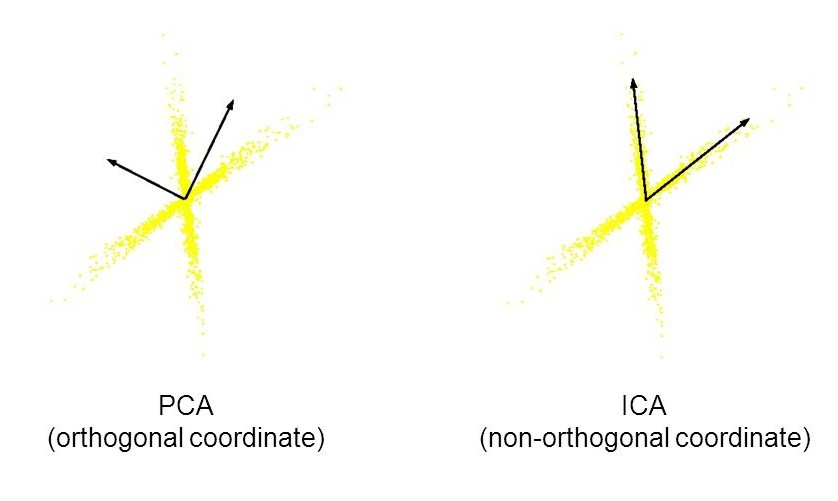
\includegraphics[width=0.75\textwidth]{ica_pca}
\end{figure}

The algorithm starts with the familiar setup: there is a matrix of observations $X$ which is assumed to be a linear mixing of latent original sources $S$: $X = S A$. 
The goal is to estimate the sources $\hat S = X W$ with $W$ being an unmixing matrix, ideally, $W = A^{-1}$.

First step is preprocessing, which is centering and "whitening" the data: demeaning data, putting it on the same scale and removing correlations in order to deal only with higher-order dependencies.
The second step can be performed with SVD: if $X = U \Sigma V^T$ is a singular value decomposition of $X$, which is already centered, we can perform whitening in the following way: \[X^\prime = \Sigma^{-1} U^\top  X\].

The Central Limit Theorem states that the sum of independent random variables tends to normal distribution under certain conditions. 
Thus, even if we only two non-Gaussian variables (which is usually the case for the signals we deal with in this problem), their sum will have the distribution closer to Gaussian than each of the original variables. 
Thus, by minimizing the normality of $X^\prime \bw$ w.r.t. $\bw$, we will be able to sequentially find the original sources and construct the unmixing matrix $W$.
This idea lies in heart of ICA.
A very simple measure of non-Gaussianity is Kurtosis. 
More advanced metrics like neg-entropy are also used frequently.

Without diving too deep into further technical details, we provide a pseudocode of FastICA algorithm [3, 9] -- a practical implementation of ICA, which we use in our experiments. For FastICA we need to select a non-linear function $f(u)$ with $g(u) = f^\prime(u)$. The typical choices are $f(u) = \log\cosh u$ and $f(u) = - e^{-\frac{u^2}{2}}$. We assume that $f$, $g$ and $g^\prime$ are vectorized, e.g. $g(\mathbf{x})$ means $\left[ g(x_1), \ldots, g(x_n) \right]^\top$.

\begin{algorithm} 
	\begin{algorithmic}
		\caption{FastICA algorithm}\label{fastica}
		\item \textbf{Input}: $X \in \mathbb{R}^{n \times d}$ -- whitened data matrix
		\item \textbf{Input}: $k \le d$ -- desired number of components
		\item \textbf{Output}: $W \in \mathbb{R}^{k \times d}$ -- unmixing matrix
		\item \textbf{Output}: $S \in \mathbb{R}^{n \times d}$ -- estimated original sources matrix
		
		\Function{FastICA}{$X, k$}
		\For{p \textbf{in} 1 to $k$}
		\State{$\bw_p \gets $ random vector of length $d$}
		\While{$\bw_p$ changes}
		\State{$\bw_p \gets 
			\frac{1}{d} X^\top g(X \bw_p)^\top - 
			\frac{1}{d} \bw_p \mathbf{1}_n^\top g^\prime(X \bw_p) $
		} \Comment{Main step}
		\State{$\bw_p \gets 
			\bw_p - \sum_{j=1}^{p-1}(\bw_p^\top \bw_j) \bw_j$
		} \Comment{Orthogonalization in order not}
		\State{$\bw_p \gets 
			\frac{ \bw_p }{ \|\bw_p \| }$
		} \Comment{to run into any of previous $\bw_j$}
		\EndWhile
		\EndFor
		\State{\textbf{output} $W$ $\gets \left[ \mathbf{w}_1, \ldots, \mathbf{w}_d \right]$ }
		\State{\textbf{output} S $\gets X W$}
		\EndFunction
		
	\end{algorithmic}
\end{algorithm}

\subsection{NMF}

Non-negative matrix factorization is another method often recommended to use to perform blind source separation.

\end{document}